\documentclass[twoside]{book}

% Packages required by doxygen
\usepackage{fixltx2e}
\usepackage{calc}
\usepackage{doxygen}
\usepackage[export]{adjustbox} % also loads graphicx
\usepackage{graphicx}
\usepackage[utf8]{inputenc}
\usepackage{makeidx}
\usepackage{multicol}
\usepackage{multirow}
\PassOptionsToPackage{warn}{textcomp}
\usepackage{textcomp}
\usepackage[nointegrals]{wasysym}
\usepackage[table]{xcolor}

% NLS support packages
\usepackage[ngerman]{babel}

% Font selection
\usepackage[T1]{fontenc}
\usepackage[scaled=.90]{helvet}
\usepackage{courier}
\usepackage{amssymb}
\usepackage{sectsty}
\renewcommand{\familydefault}{\sfdefault}
\allsectionsfont{%
  \fontseries{bc}\selectfont%
  \color{darkgray}%
}
\renewcommand{\DoxyLabelFont}{%
  \fontseries{bc}\selectfont%
  \color{darkgray}%
}
\newcommand{\+}{\discretionary{\mbox{\scriptsize$\hookleftarrow$}}{}{}}

% Page & text layout
\usepackage{geometry}
\geometry{%
  a4paper,%
  top=2.5cm,%
  bottom=2.5cm,%
  left=2.5cm,%
  right=2.5cm%
}
\tolerance=750
\hfuzz=15pt
\hbadness=750
\setlength{\emergencystretch}{15pt}
\setlength{\parindent}{0cm}
\setlength{\parskip}{3ex plus 2ex minus 2ex}
\makeatletter
\renewcommand{\paragraph}{%
  \@startsection{paragraph}{4}{0ex}{-1.0ex}{1.0ex}{%
    \normalfont\normalsize\bfseries\SS@parafont%
  }%
}
\renewcommand{\subparagraph}{%
  \@startsection{subparagraph}{5}{0ex}{-1.0ex}{1.0ex}{%
    \normalfont\normalsize\bfseries\SS@subparafont%
  }%
}
\makeatother

% Headers & footers
\usepackage{fancyhdr}
\pagestyle{fancyplain}
\fancyhead[LE]{\fancyplain{}{\bfseries\thepage}}
\fancyhead[CE]{\fancyplain{}{}}
\fancyhead[RE]{\fancyplain{}{\bfseries\leftmark}}
\fancyhead[LO]{\fancyplain{}{\bfseries\rightmark}}
\fancyhead[CO]{\fancyplain{}{}}
\fancyhead[RO]{\fancyplain{}{\bfseries\thepage}}
\fancyfoot[LE]{\fancyplain{}{}}
\fancyfoot[CE]{\fancyplain{}{}}
\fancyfoot[RE]{\fancyplain{}{\bfseries\scriptsize Erzeugt von Doxygen }}
\fancyfoot[LO]{\fancyplain{}{\bfseries\scriptsize Erzeugt von Doxygen }}
\fancyfoot[CO]{\fancyplain{}{}}
\fancyfoot[RO]{\fancyplain{}{}}
\renewcommand{\footrulewidth}{0.4pt}
\renewcommand{\chaptermark}[1]{%
  \markboth{#1}{}%
}
\renewcommand{\sectionmark}[1]{%
  \markright{\thesection\ #1}%
}

% Indices & bibliography
\usepackage{natbib}
\usepackage[titles]{tocloft}
\setcounter{tocdepth}{3}
\setcounter{secnumdepth}{5}
\makeindex

% Custom commands
\newcommand{\clearemptydoublepage}{%
  \newpage{\pagestyle{empty}\cleardoublepage}%
}

\usepackage{caption}
\captionsetup{labelsep=space,justification=centering,font={bf},singlelinecheck=off,skip=4pt,position=top}

%===== C O N T E N T S =====

\begin{document}

% Titlepage & ToC
\pagenumbering{alph}
\begin{titlepage}
\vspace*{7cm}
\begin{center}%
{\Large Abschlussprojekt }\\
\vspace*{1cm}
{\large Erzeugt von Doxygen 1.8.13}\\
\end{center}
\end{titlepage}
\clearemptydoublepage
\pagenumbering{roman}
\tableofcontents
\clearemptydoublepage
\pagenumbering{arabic}

%--- Begin generated contents ---
\chapter{Datei-\/\+Verzeichnis}
\section{Auflistung der Dateien}
Hier folgt die Aufzählung aller Dateien mit einer Kurzbeschreibung\+:\begin{DoxyCompactList}
\item\contentsline{section}{/home/zero/abschlussprojekt/\hyperlink{abschlussprojekt_8c}{abschlussprojekt.\+c} }{\pageref{abschlussprojekt_8c}}{}
\item\contentsline{section}{/home/zero/abschlussprojekt/\hyperlink{make__string_8cpp}{make\+\_\+string.\+cpp} }{\pageref{make__string_8cpp}}{}
\item\contentsline{section}{/home/zero/abschlussprojekt/\hyperlink{make__string_8h}{make\+\_\+string.\+h} }{\pageref{make__string_8h}}{}
\item\contentsline{section}{/home/zero/abschlussprojekt/\hyperlink{makros_8h}{makros.\+h} }{\pageref{makros_8h}}{}
\item\contentsline{section}{/home/zero/abschlussprojekt/\hyperlink{pumpe__1_8cpp}{pumpe\+\_\+1.\+cpp} }{\pageref{pumpe__1_8cpp}}{}
\item\contentsline{section}{/home/zero/abschlussprojekt/\hyperlink{pumpe__1_8h}{pumpe\+\_\+1.\+h} }{\pageref{pumpe__1_8h}}{}
\item\contentsline{section}{/home/zero/abschlussprojekt/\hyperlink{pumpe__2_8cpp}{pumpe\+\_\+2.\+cpp} }{\pageref{pumpe__2_8cpp}}{}
\item\contentsline{section}{/home/zero/abschlussprojekt/\hyperlink{pumpe__2_8h}{pumpe\+\_\+2.\+h} }{\pageref{pumpe__2_8h}}{}
\item\contentsline{section}{/home/zero/abschlussprojekt/\hyperlink{tuer__zu_8cpp}{tuer\+\_\+zu.\+cpp} }{\pageref{tuer__zu_8cpp}}{}
\item\contentsline{section}{/home/zero/abschlussprojekt/\hyperlink{tuer__zu_8h}{tuer\+\_\+zu.\+h} }{\pageref{tuer__zu_8h}}{}
\item\contentsline{section}{/home/zero/abschlussprojekt/\hyperlink{update__lcd_8h}{update\+\_\+lcd.\+h} }{\pageref{update__lcd_8h}}{}
\item\contentsline{section}{/home/zero/abschlussprojekt/\hyperlink{update__limits_8cpp}{update\+\_\+limits.\+cpp} }{\pageref{update__limits_8cpp}}{}
\item\contentsline{section}{/home/zero/abschlussprojekt/\hyperlink{update__limits_8h}{update\+\_\+limits.\+h} }{\pageref{update__limits_8h}}{}
\item\contentsline{section}{/home/zero/abschlussprojekt/\hyperlink{update__messwerte_8h}{update\+\_\+messwerte.\+h} }{\pageref{update__messwerte_8h}}{}
\end{DoxyCompactList}

\chapter{Datei-\/\+Dokumentation}
\section{abschlussprojekt\+\_\+doxygen.\+c-\/\+Dateireferenz}
\label{abschlussprojekt__doxygen_8c}\index{abschlussprojekt\+\_\+doxygen.\+c@{abschlussprojekt\+\_\+doxygen.\+c}}
{\ttfamily \#include \char`\"{}D\+H\+T.\+h\char`\"{}}\newline
{\ttfamily \#include $<$Wire.\+h$>$}\newline
{\ttfamily \#include $<$Liquid\+Crystal\+\_\+\+I2\+C.\+h$>$}\newline
Include-\/\+Abhängigkeitsdiagramm für abschlussprojekt\+\_\+doxygen.\+c\+:\nopagebreak
\begin{figure}[H]
\begin{center}
\leavevmode
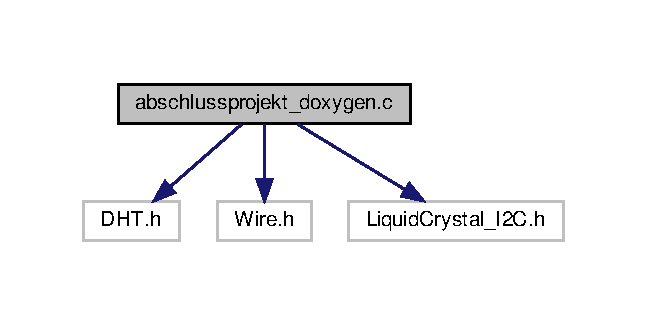
\includegraphics[width=311pt]{abschlussprojekt__doxygen_8c__incl}
\end{center}
\end{figure}
\subsection*{Makrodefinitionen}
\begin{DoxyCompactItemize}
\item 
\#define \textbf{ D\+H\+T\+T\+Y\+PE}~D\+H\+T22
\item 
\#define \textbf{ T\+A\+S\+T\+E\+R\+\_\+\+D\+I\+S\+P\+L\+AY}~2
\item 
\#define \textbf{ R\+E\+L\+A\+I\+S\+\_\+\+P\+U\+M\+P\+E\+\_\+\+O\+B\+EN}~4
\item 
\#define \textbf{ R\+E\+L\+A\+I\+S\+\_\+\+P\+U\+M\+P\+E\+\_\+\+U\+N\+T\+EN}~5
\item 
\#define \textbf{ R\+E\+L\+A\+I\+S\+\_\+\+L\+U\+E\+F\+T\+ER}~6
\item 
\#define \textbf{ R\+E\+L\+A\+I\+S\+\_\+\+U\+V\+\_\+\+L\+ED}~7
\item 
\#define \textbf{ R\+E\+L\+A\+I\+S\+\_\+\+H\+E\+I\+Z\+U\+NG}~8
\item 
\#define \textbf{ T\+E\+M\+P\+E\+R\+A\+T\+U\+R\+S\+E\+N\+S\+O\+R\+\_\+\+L\+U\+E\+F\+T\+ER}~9
\item 
\#define \textbf{ H\+E\+L\+L\+I\+G\+K\+E\+I\+T\+S\+S\+E\+N\+S\+OR}~10
\item 
\#define \textbf{ R\+E\+E\+D\+K\+O\+N\+T\+A\+KT}~11
\item 
\#define \textbf{ E\+R\+D\+F\+E\+U\+C\+H\+T\+E\+S\+E\+N\+S\+O\+R\+\_\+1}~A0
\item 
\#define \textbf{ E\+R\+D\+F\+E\+U\+C\+H\+T\+E\+S\+E\+N\+S\+O\+R\+\_\+2}~A1
\item 
\#define \textbf{ L\+I\+M\+I\+T\+\_\+\+E\+R\+D\+F\+E\+U\+C\+H\+T\+E\+\_\+1}~A2
\item 
\#define \textbf{ L\+I\+M\+I\+T\+\_\+\+E\+R\+D\+F\+E\+U\+C\+H\+T\+E\+\_\+2}~A3
\item 
\#define \textbf{ L\+I\+M\+I\+T\+\_\+\+T\+E\+M\+P\+E\+R\+A\+T\+UR}~A6
\item 
\#define \textbf{ L\+I\+M\+I\+T\+\_\+\+L\+U\+E\+F\+T\+ER}~A5
\item 
\#define \textbf{ zustand\+\_\+warten\+\_\+zu\+\_\+trocken}~0
\item 
\#define \textbf{ zustand\+\_\+pumpt}~1
\item 
\#define \textbf{ zustand\+\_\+warten\+\_\+durchfeuchtung}~2
\end{DoxyCompactItemize}
\subsection*{Funktionen}
\begin{DoxyCompactItemize}
\item 
Liquid\+Crystal\+\_\+\+I2C \textbf{ lcd} (0x3\+F, 20, 4)
\item 
D\+HT \textbf{ dht} (\textbf{ T\+E\+M\+P\+E\+R\+A\+T\+U\+R\+S\+E\+N\+S\+O\+R\+\_\+\+L\+U\+E\+F\+T\+ER}, \textbf{ D\+H\+T\+T\+Y\+PE})
\item 
String \textbf{ make\+\_\+string} (String s)
\item 
void \textbf{ update\+\_\+messwerte} ()
\item 
void \textbf{ update\+\_\+limits} ()
\item 
bool \textbf{ tuer\+\_\+zu} ()
\item 
void \textbf{ update\+\_\+lcd} (int nr\+\_\+display, int \textbf{ temp\+\_\+luft\+\_\+C}, int \textbf{ hum\+\_\+luft}, int \textbf{ hum\+\_\+erde\+\_\+1\+\_\+adc}, int \textbf{ hum\+\_\+erde\+\_\+2\+\_\+adc}, int \textbf{ limit\+\_\+feuchte\+\_\+1\+\_\+adc}, int \textbf{ limit\+\_\+feuchte\+\_\+2\+\_\+adc}, int \textbf{ limit\+\_\+temp\+\_\+adc}, int \textbf{ limit\+\_\+luefter\+\_\+adc})
\item 
void \textbf{ setup} ()
\item 
void \textbf{ loop} ()
\end{DoxyCompactItemize}
\subsection*{Variablen}
\begin{DoxyCompactItemize}
\item 
unsigned long \textbf{ t0\+\_\+temperaturmessung}
\item 
unsigned long \textbf{ dt\+\_\+temperaturmessung\+\_\+ms} = 2000
\item 
unsigned long \textbf{ t0\+\_\+display}
\item 
unsigned long \textbf{ dt\+\_\+display\+\_\+ms} = 2000
\item 
unsigned long \textbf{ t0\+\_\+erdfeuchtemessung}
\item 
unsigned long \textbf{ dt\+\_\+erdfeuchtemessung\+\_\+ms} = 5000
\item 
unsigned long \textbf{ t0\+\_\+pumpe\+\_\+1}
\item 
unsigned long \textbf{ dt\+\_\+pumpendauer\+\_\+1\+\_\+ms} = 5000
\item 
unsigned long \textbf{ t0\+\_\+pumpe\+\_\+2}
\item 
unsigned long \textbf{ dt\+\_\+pumpendauer\+\_\+2\+\_\+ms} = 5000
\item 
unsigned long \textbf{ t0\+\_\+durchfeuchtung\+\_\+1}
\item 
unsigned long \textbf{ dt\+\_\+warten\+\_\+durchfeuchtung\+\_\+1\+\_\+ms} = 10000
\item 
unsigned long \textbf{ t0\+\_\+durchfeuchtung\+\_\+2}
\item 
unsigned long \textbf{ dt\+\_\+warten\+\_\+durchfeuchtung\+\_\+2\+\_\+ms} = 10000
\item 
unsigned long \textbf{ t0\+\_\+heizung}
\item 
unsigned long \textbf{ dt\+\_\+heizung\+\_\+ms} = 5000
\item 
unsigned long \textbf{ t0\+\_\+luefter}
\item 
unsigned long \textbf{ dt\+\_\+luefter\+\_\+ms} = 5000
\item 
unsigned long \textbf{ t0\+\_\+helligkeit}
\item 
unsigned long \textbf{ dt\+\_\+helligkeit\+\_\+ms} = 5000
\item 
int \textbf{ hum\+\_\+erde\+\_\+1\+\_\+adc}
\item 
int \textbf{ hum\+\_\+erde\+\_\+2\+\_\+adc}
\item 
int \textbf{ hum\+\_\+luft}
\item 
int \textbf{ temp\+\_\+luft\+\_\+C}
\item 
int \textbf{ limit\+\_\+feuchte\+\_\+1\+\_\+adc}
\item 
int \textbf{ limit\+\_\+feuchte\+\_\+2\+\_\+adc}
\item 
int \textbf{ limit\+\_\+temp\+\_\+adc}
\item 
int \textbf{ limit\+\_\+temp\+\_\+C}
\item 
int \textbf{ limit\+\_\+luefter\+\_\+adc}
\item 
int \textbf{ limit\+\_\+luefter\+\_\+C} = 15
\item 
int \textbf{ zustand\+\_\+1} = \textbf{ zustand\+\_\+warten\+\_\+zu\+\_\+trocken}
\item 
int \textbf{ zustand\+\_\+2} = \textbf{ zustand\+\_\+warten\+\_\+zu\+\_\+trocken}
\item 
int \textbf{ voriger\+\_\+taster}
\item 
int \textbf{ aktueller\+\_\+taster} = L\+OW
\item 
int \textbf{ displ\+\_\+nr} = 0
\end{DoxyCompactItemize}


\subsection{Makro-\/\+Dokumentation}
\mbox{\label{abschlussprojekt__doxygen_8c_a2c509dba12bba99883a5be9341b7a0c5}} 
\index{abschlussprojekt\+\_\+doxygen.\+c@{abschlussprojekt\+\_\+doxygen.\+c}!D\+H\+T\+T\+Y\+PE@{D\+H\+T\+T\+Y\+PE}}
\index{D\+H\+T\+T\+Y\+PE@{D\+H\+T\+T\+Y\+PE}!abschlussprojekt\+\_\+doxygen.\+c@{abschlussprojekt\+\_\+doxygen.\+c}}
\subsubsection{D\+H\+T\+T\+Y\+PE}
{\footnotesize\ttfamily \#define D\+H\+T\+T\+Y\+PE~D\+H\+T22}



Definiert in Zeile 23 der Datei abschlussprojekt\+\_\+doxygen.\+c.

\mbox{\label{abschlussprojekt__doxygen_8c_a217a0b1523cc63a0e9618b0b9bcc3944}} 
\index{abschlussprojekt\+\_\+doxygen.\+c@{abschlussprojekt\+\_\+doxygen.\+c}!E\+R\+D\+F\+E\+U\+C\+H\+T\+E\+S\+E\+N\+S\+O\+R\+\_\+1@{E\+R\+D\+F\+E\+U\+C\+H\+T\+E\+S\+E\+N\+S\+O\+R\+\_\+1}}
\index{E\+R\+D\+F\+E\+U\+C\+H\+T\+E\+S\+E\+N\+S\+O\+R\+\_\+1@{E\+R\+D\+F\+E\+U\+C\+H\+T\+E\+S\+E\+N\+S\+O\+R\+\_\+1}!abschlussprojekt\+\_\+doxygen.\+c@{abschlussprojekt\+\_\+doxygen.\+c}}
\subsubsection{E\+R\+D\+F\+E\+U\+C\+H\+T\+E\+S\+E\+N\+S\+O\+R\+\_\+1}
{\footnotesize\ttfamily \#define E\+R\+D\+F\+E\+U\+C\+H\+T\+E\+S\+E\+N\+S\+O\+R\+\_\+1~A0}



Definiert in Zeile 35 der Datei abschlussprojekt\+\_\+doxygen.\+c.

\mbox{\label{abschlussprojekt__doxygen_8c_ab35f6b04d1873122637b48a378828072}} 
\index{abschlussprojekt\+\_\+doxygen.\+c@{abschlussprojekt\+\_\+doxygen.\+c}!E\+R\+D\+F\+E\+U\+C\+H\+T\+E\+S\+E\+N\+S\+O\+R\+\_\+2@{E\+R\+D\+F\+E\+U\+C\+H\+T\+E\+S\+E\+N\+S\+O\+R\+\_\+2}}
\index{E\+R\+D\+F\+E\+U\+C\+H\+T\+E\+S\+E\+N\+S\+O\+R\+\_\+2@{E\+R\+D\+F\+E\+U\+C\+H\+T\+E\+S\+E\+N\+S\+O\+R\+\_\+2}!abschlussprojekt\+\_\+doxygen.\+c@{abschlussprojekt\+\_\+doxygen.\+c}}
\subsubsection{E\+R\+D\+F\+E\+U\+C\+H\+T\+E\+S\+E\+N\+S\+O\+R\+\_\+2}
{\footnotesize\ttfamily \#define E\+R\+D\+F\+E\+U\+C\+H\+T\+E\+S\+E\+N\+S\+O\+R\+\_\+2~A1}



Definiert in Zeile 36 der Datei abschlussprojekt\+\_\+doxygen.\+c.

\mbox{\label{abschlussprojekt__doxygen_8c_abd1dbbe0460847d74097b3fbb78d9457}} 
\index{abschlussprojekt\+\_\+doxygen.\+c@{abschlussprojekt\+\_\+doxygen.\+c}!H\+E\+L\+L\+I\+G\+K\+E\+I\+T\+S\+S\+E\+N\+S\+OR@{H\+E\+L\+L\+I\+G\+K\+E\+I\+T\+S\+S\+E\+N\+S\+OR}}
\index{H\+E\+L\+L\+I\+G\+K\+E\+I\+T\+S\+S\+E\+N\+S\+OR@{H\+E\+L\+L\+I\+G\+K\+E\+I\+T\+S\+S\+E\+N\+S\+OR}!abschlussprojekt\+\_\+doxygen.\+c@{abschlussprojekt\+\_\+doxygen.\+c}}
\subsubsection{H\+E\+L\+L\+I\+G\+K\+E\+I\+T\+S\+S\+E\+N\+S\+OR}
{\footnotesize\ttfamily \#define H\+E\+L\+L\+I\+G\+K\+E\+I\+T\+S\+S\+E\+N\+S\+OR~10}



Definiert in Zeile 31 der Datei abschlussprojekt\+\_\+doxygen.\+c.

\mbox{\label{abschlussprojekt__doxygen_8c_a2cfb9232ef93fe3dbe489ea0ed78ab5c}} 
\index{abschlussprojekt\+\_\+doxygen.\+c@{abschlussprojekt\+\_\+doxygen.\+c}!L\+I\+M\+I\+T\+\_\+\+E\+R\+D\+F\+E\+U\+C\+H\+T\+E\+\_\+1@{L\+I\+M\+I\+T\+\_\+\+E\+R\+D\+F\+E\+U\+C\+H\+T\+E\+\_\+1}}
\index{L\+I\+M\+I\+T\+\_\+\+E\+R\+D\+F\+E\+U\+C\+H\+T\+E\+\_\+1@{L\+I\+M\+I\+T\+\_\+\+E\+R\+D\+F\+E\+U\+C\+H\+T\+E\+\_\+1}!abschlussprojekt\+\_\+doxygen.\+c@{abschlussprojekt\+\_\+doxygen.\+c}}
\subsubsection{L\+I\+M\+I\+T\+\_\+\+E\+R\+D\+F\+E\+U\+C\+H\+T\+E\+\_\+1}
{\footnotesize\ttfamily \#define L\+I\+M\+I\+T\+\_\+\+E\+R\+D\+F\+E\+U\+C\+H\+T\+E\+\_\+1~A2}



Definiert in Zeile 37 der Datei abschlussprojekt\+\_\+doxygen.\+c.

\mbox{\label{abschlussprojekt__doxygen_8c_a06863b5c4eac468b904afed8c6c36440}} 
\index{abschlussprojekt\+\_\+doxygen.\+c@{abschlussprojekt\+\_\+doxygen.\+c}!L\+I\+M\+I\+T\+\_\+\+E\+R\+D\+F\+E\+U\+C\+H\+T\+E\+\_\+2@{L\+I\+M\+I\+T\+\_\+\+E\+R\+D\+F\+E\+U\+C\+H\+T\+E\+\_\+2}}
\index{L\+I\+M\+I\+T\+\_\+\+E\+R\+D\+F\+E\+U\+C\+H\+T\+E\+\_\+2@{L\+I\+M\+I\+T\+\_\+\+E\+R\+D\+F\+E\+U\+C\+H\+T\+E\+\_\+2}!abschlussprojekt\+\_\+doxygen.\+c@{abschlussprojekt\+\_\+doxygen.\+c}}
\subsubsection{L\+I\+M\+I\+T\+\_\+\+E\+R\+D\+F\+E\+U\+C\+H\+T\+E\+\_\+2}
{\footnotesize\ttfamily \#define L\+I\+M\+I\+T\+\_\+\+E\+R\+D\+F\+E\+U\+C\+H\+T\+E\+\_\+2~A3}



Definiert in Zeile 38 der Datei abschlussprojekt\+\_\+doxygen.\+c.

\mbox{\label{abschlussprojekt__doxygen_8c_a392b9a22bb52d29603ffb57ab4255e86}} 
\index{abschlussprojekt\+\_\+doxygen.\+c@{abschlussprojekt\+\_\+doxygen.\+c}!L\+I\+M\+I\+T\+\_\+\+L\+U\+E\+F\+T\+ER@{L\+I\+M\+I\+T\+\_\+\+L\+U\+E\+F\+T\+ER}}
\index{L\+I\+M\+I\+T\+\_\+\+L\+U\+E\+F\+T\+ER@{L\+I\+M\+I\+T\+\_\+\+L\+U\+E\+F\+T\+ER}!abschlussprojekt\+\_\+doxygen.\+c@{abschlussprojekt\+\_\+doxygen.\+c}}
\subsubsection{L\+I\+M\+I\+T\+\_\+\+L\+U\+E\+F\+T\+ER}
{\footnotesize\ttfamily \#define L\+I\+M\+I\+T\+\_\+\+L\+U\+E\+F\+T\+ER~A5}



Definiert in Zeile 40 der Datei abschlussprojekt\+\_\+doxygen.\+c.

\mbox{\label{abschlussprojekt__doxygen_8c_ae07fe35374a1fd6e6d921bd39ba73b99}} 
\index{abschlussprojekt\+\_\+doxygen.\+c@{abschlussprojekt\+\_\+doxygen.\+c}!L\+I\+M\+I\+T\+\_\+\+T\+E\+M\+P\+E\+R\+A\+T\+UR@{L\+I\+M\+I\+T\+\_\+\+T\+E\+M\+P\+E\+R\+A\+T\+UR}}
\index{L\+I\+M\+I\+T\+\_\+\+T\+E\+M\+P\+E\+R\+A\+T\+UR@{L\+I\+M\+I\+T\+\_\+\+T\+E\+M\+P\+E\+R\+A\+T\+UR}!abschlussprojekt\+\_\+doxygen.\+c@{abschlussprojekt\+\_\+doxygen.\+c}}
\subsubsection{L\+I\+M\+I\+T\+\_\+\+T\+E\+M\+P\+E\+R\+A\+T\+UR}
{\footnotesize\ttfamily \#define L\+I\+M\+I\+T\+\_\+\+T\+E\+M\+P\+E\+R\+A\+T\+UR~A6}



Definiert in Zeile 39 der Datei abschlussprojekt\+\_\+doxygen.\+c.

\mbox{\label{abschlussprojekt__doxygen_8c_aa5c8a88c5a3dde80789f0b329b877a6f}} 
\index{abschlussprojekt\+\_\+doxygen.\+c@{abschlussprojekt\+\_\+doxygen.\+c}!R\+E\+E\+D\+K\+O\+N\+T\+A\+KT@{R\+E\+E\+D\+K\+O\+N\+T\+A\+KT}}
\index{R\+E\+E\+D\+K\+O\+N\+T\+A\+KT@{R\+E\+E\+D\+K\+O\+N\+T\+A\+KT}!abschlussprojekt\+\_\+doxygen.\+c@{abschlussprojekt\+\_\+doxygen.\+c}}
\subsubsection{R\+E\+E\+D\+K\+O\+N\+T\+A\+KT}
{\footnotesize\ttfamily \#define R\+E\+E\+D\+K\+O\+N\+T\+A\+KT~11}



Definiert in Zeile 32 der Datei abschlussprojekt\+\_\+doxygen.\+c.

\mbox{\label{abschlussprojekt__doxygen_8c_a2fc336b6f27547c3b2f8e501806d95e2}} 
\index{abschlussprojekt\+\_\+doxygen.\+c@{abschlussprojekt\+\_\+doxygen.\+c}!R\+E\+L\+A\+I\+S\+\_\+\+H\+E\+I\+Z\+U\+NG@{R\+E\+L\+A\+I\+S\+\_\+\+H\+E\+I\+Z\+U\+NG}}
\index{R\+E\+L\+A\+I\+S\+\_\+\+H\+E\+I\+Z\+U\+NG@{R\+E\+L\+A\+I\+S\+\_\+\+H\+E\+I\+Z\+U\+NG}!abschlussprojekt\+\_\+doxygen.\+c@{abschlussprojekt\+\_\+doxygen.\+c}}
\subsubsection{R\+E\+L\+A\+I\+S\+\_\+\+H\+E\+I\+Z\+U\+NG}
{\footnotesize\ttfamily \#define R\+E\+L\+A\+I\+S\+\_\+\+H\+E\+I\+Z\+U\+NG~8}



Definiert in Zeile 29 der Datei abschlussprojekt\+\_\+doxygen.\+c.

\mbox{\label{abschlussprojekt__doxygen_8c_a30d6fbf03c0e3ae5cf71977fe9dfa1d5}} 
\index{abschlussprojekt\+\_\+doxygen.\+c@{abschlussprojekt\+\_\+doxygen.\+c}!R\+E\+L\+A\+I\+S\+\_\+\+L\+U\+E\+F\+T\+ER@{R\+E\+L\+A\+I\+S\+\_\+\+L\+U\+E\+F\+T\+ER}}
\index{R\+E\+L\+A\+I\+S\+\_\+\+L\+U\+E\+F\+T\+ER@{R\+E\+L\+A\+I\+S\+\_\+\+L\+U\+E\+F\+T\+ER}!abschlussprojekt\+\_\+doxygen.\+c@{abschlussprojekt\+\_\+doxygen.\+c}}
\subsubsection{R\+E\+L\+A\+I\+S\+\_\+\+L\+U\+E\+F\+T\+ER}
{\footnotesize\ttfamily \#define R\+E\+L\+A\+I\+S\+\_\+\+L\+U\+E\+F\+T\+ER~6}



Definiert in Zeile 27 der Datei abschlussprojekt\+\_\+doxygen.\+c.

\mbox{\label{abschlussprojekt__doxygen_8c_ae5585e7e3d65edaff2d78517eb4f759d}} 
\index{abschlussprojekt\+\_\+doxygen.\+c@{abschlussprojekt\+\_\+doxygen.\+c}!R\+E\+L\+A\+I\+S\+\_\+\+P\+U\+M\+P\+E\+\_\+\+O\+B\+EN@{R\+E\+L\+A\+I\+S\+\_\+\+P\+U\+M\+P\+E\+\_\+\+O\+B\+EN}}
\index{R\+E\+L\+A\+I\+S\+\_\+\+P\+U\+M\+P\+E\+\_\+\+O\+B\+EN@{R\+E\+L\+A\+I\+S\+\_\+\+P\+U\+M\+P\+E\+\_\+\+O\+B\+EN}!abschlussprojekt\+\_\+doxygen.\+c@{abschlussprojekt\+\_\+doxygen.\+c}}
\subsubsection{R\+E\+L\+A\+I\+S\+\_\+\+P\+U\+M\+P\+E\+\_\+\+O\+B\+EN}
{\footnotesize\ttfamily \#define R\+E\+L\+A\+I\+S\+\_\+\+P\+U\+M\+P\+E\+\_\+\+O\+B\+EN~4}



Definiert in Zeile 25 der Datei abschlussprojekt\+\_\+doxygen.\+c.

\mbox{\label{abschlussprojekt__doxygen_8c_a2f5672d9a8ae3f2d5a148adbb8143c68}} 
\index{abschlussprojekt\+\_\+doxygen.\+c@{abschlussprojekt\+\_\+doxygen.\+c}!R\+E\+L\+A\+I\+S\+\_\+\+P\+U\+M\+P\+E\+\_\+\+U\+N\+T\+EN@{R\+E\+L\+A\+I\+S\+\_\+\+P\+U\+M\+P\+E\+\_\+\+U\+N\+T\+EN}}
\index{R\+E\+L\+A\+I\+S\+\_\+\+P\+U\+M\+P\+E\+\_\+\+U\+N\+T\+EN@{R\+E\+L\+A\+I\+S\+\_\+\+P\+U\+M\+P\+E\+\_\+\+U\+N\+T\+EN}!abschlussprojekt\+\_\+doxygen.\+c@{abschlussprojekt\+\_\+doxygen.\+c}}
\subsubsection{R\+E\+L\+A\+I\+S\+\_\+\+P\+U\+M\+P\+E\+\_\+\+U\+N\+T\+EN}
{\footnotesize\ttfamily \#define R\+E\+L\+A\+I\+S\+\_\+\+P\+U\+M\+P\+E\+\_\+\+U\+N\+T\+EN~5}



Definiert in Zeile 26 der Datei abschlussprojekt\+\_\+doxygen.\+c.

\mbox{\label{abschlussprojekt__doxygen_8c_a5316bb60c0bf0c793c28ba8815caa69b}} 
\index{abschlussprojekt\+\_\+doxygen.\+c@{abschlussprojekt\+\_\+doxygen.\+c}!R\+E\+L\+A\+I\+S\+\_\+\+U\+V\+\_\+\+L\+ED@{R\+E\+L\+A\+I\+S\+\_\+\+U\+V\+\_\+\+L\+ED}}
\index{R\+E\+L\+A\+I\+S\+\_\+\+U\+V\+\_\+\+L\+ED@{R\+E\+L\+A\+I\+S\+\_\+\+U\+V\+\_\+\+L\+ED}!abschlussprojekt\+\_\+doxygen.\+c@{abschlussprojekt\+\_\+doxygen.\+c}}
\subsubsection{R\+E\+L\+A\+I\+S\+\_\+\+U\+V\+\_\+\+L\+ED}
{\footnotesize\ttfamily \#define R\+E\+L\+A\+I\+S\+\_\+\+U\+V\+\_\+\+L\+ED~7}



Definiert in Zeile 28 der Datei abschlussprojekt\+\_\+doxygen.\+c.

\mbox{\label{abschlussprojekt__doxygen_8c_a3edd9adbe80cfa6949a85935a79275d7}} 
\index{abschlussprojekt\+\_\+doxygen.\+c@{abschlussprojekt\+\_\+doxygen.\+c}!T\+A\+S\+T\+E\+R\+\_\+\+D\+I\+S\+P\+L\+AY@{T\+A\+S\+T\+E\+R\+\_\+\+D\+I\+S\+P\+L\+AY}}
\index{T\+A\+S\+T\+E\+R\+\_\+\+D\+I\+S\+P\+L\+AY@{T\+A\+S\+T\+E\+R\+\_\+\+D\+I\+S\+P\+L\+AY}!abschlussprojekt\+\_\+doxygen.\+c@{abschlussprojekt\+\_\+doxygen.\+c}}
\subsubsection{T\+A\+S\+T\+E\+R\+\_\+\+D\+I\+S\+P\+L\+AY}
{\footnotesize\ttfamily \#define T\+A\+S\+T\+E\+R\+\_\+\+D\+I\+S\+P\+L\+AY~2}



Definiert in Zeile 24 der Datei abschlussprojekt\+\_\+doxygen.\+c.

\mbox{\label{abschlussprojekt__doxygen_8c_a9894c05769fdf48b3506408030591a65}} 
\index{abschlussprojekt\+\_\+doxygen.\+c@{abschlussprojekt\+\_\+doxygen.\+c}!T\+E\+M\+P\+E\+R\+A\+T\+U\+R\+S\+E\+N\+S\+O\+R\+\_\+\+L\+U\+E\+F\+T\+ER@{T\+E\+M\+P\+E\+R\+A\+T\+U\+R\+S\+E\+N\+S\+O\+R\+\_\+\+L\+U\+E\+F\+T\+ER}}
\index{T\+E\+M\+P\+E\+R\+A\+T\+U\+R\+S\+E\+N\+S\+O\+R\+\_\+\+L\+U\+E\+F\+T\+ER@{T\+E\+M\+P\+E\+R\+A\+T\+U\+R\+S\+E\+N\+S\+O\+R\+\_\+\+L\+U\+E\+F\+T\+ER}!abschlussprojekt\+\_\+doxygen.\+c@{abschlussprojekt\+\_\+doxygen.\+c}}
\subsubsection{T\+E\+M\+P\+E\+R\+A\+T\+U\+R\+S\+E\+N\+S\+O\+R\+\_\+\+L\+U\+E\+F\+T\+ER}
{\footnotesize\ttfamily \#define T\+E\+M\+P\+E\+R\+A\+T\+U\+R\+S\+E\+N\+S\+O\+R\+\_\+\+L\+U\+E\+F\+T\+ER~9}



Definiert in Zeile 30 der Datei abschlussprojekt\+\_\+doxygen.\+c.

\mbox{\label{abschlussprojekt__doxygen_8c_a451a24326bd3759cea1cbd0da8d4bb12}} 
\index{abschlussprojekt\+\_\+doxygen.\+c@{abschlussprojekt\+\_\+doxygen.\+c}!zustand\+\_\+pumpt@{zustand\+\_\+pumpt}}
\index{zustand\+\_\+pumpt@{zustand\+\_\+pumpt}!abschlussprojekt\+\_\+doxygen.\+c@{abschlussprojekt\+\_\+doxygen.\+c}}
\subsubsection{zustand\+\_\+pumpt}
{\footnotesize\ttfamily \#define zustand\+\_\+pumpt~1}



Definiert in Zeile 92 der Datei abschlussprojekt\+\_\+doxygen.\+c.

\mbox{\label{abschlussprojekt__doxygen_8c_a15e9e3e52a86bfb566502710f2453c20}} 
\index{abschlussprojekt\+\_\+doxygen.\+c@{abschlussprojekt\+\_\+doxygen.\+c}!zustand\+\_\+warten\+\_\+durchfeuchtung@{zustand\+\_\+warten\+\_\+durchfeuchtung}}
\index{zustand\+\_\+warten\+\_\+durchfeuchtung@{zustand\+\_\+warten\+\_\+durchfeuchtung}!abschlussprojekt\+\_\+doxygen.\+c@{abschlussprojekt\+\_\+doxygen.\+c}}
\subsubsection{zustand\+\_\+warten\+\_\+durchfeuchtung}
{\footnotesize\ttfamily \#define zustand\+\_\+warten\+\_\+durchfeuchtung~2}



Definiert in Zeile 93 der Datei abschlussprojekt\+\_\+doxygen.\+c.

\mbox{\label{abschlussprojekt__doxygen_8c_acd99f73b20037e5fcba7a4a031e0f320}} 
\index{abschlussprojekt\+\_\+doxygen.\+c@{abschlussprojekt\+\_\+doxygen.\+c}!zustand\+\_\+warten\+\_\+zu\+\_\+trocken@{zustand\+\_\+warten\+\_\+zu\+\_\+trocken}}
\index{zustand\+\_\+warten\+\_\+zu\+\_\+trocken@{zustand\+\_\+warten\+\_\+zu\+\_\+trocken}!abschlussprojekt\+\_\+doxygen.\+c@{abschlussprojekt\+\_\+doxygen.\+c}}
\subsubsection{zustand\+\_\+warten\+\_\+zu\+\_\+trocken}
{\footnotesize\ttfamily \#define zustand\+\_\+warten\+\_\+zu\+\_\+trocken~0}



Definiert in Zeile 91 der Datei abschlussprojekt\+\_\+doxygen.\+c.



\subsection{Dokumentation der Funktionen}
\mbox{\label{abschlussprojekt__doxygen_8c_a94f388d273b0cbe6d7f3c0d5817f688b}} 
\index{abschlussprojekt\+\_\+doxygen.\+c@{abschlussprojekt\+\_\+doxygen.\+c}!dht@{dht}}
\index{dht@{dht}!abschlussprojekt\+\_\+doxygen.\+c@{abschlussprojekt\+\_\+doxygen.\+c}}
\subsubsection{dht()}
{\footnotesize\ttfamily D\+HT dht (\begin{DoxyParamCaption}\item[{\textbf{ T\+E\+M\+P\+E\+R\+A\+T\+U\+R\+S\+E\+N\+S\+O\+R\+\_\+\+L\+U\+E\+F\+T\+ER}}]{,  }\item[{\textbf{ D\+H\+T\+T\+Y\+PE}}]{ }\end{DoxyParamCaption})}

\mbox{\label{abschlussprojekt__doxygen_8c_a7392e8043ba37d68cf0d13e0264acd85}} 
\index{abschlussprojekt\+\_\+doxygen.\+c@{abschlussprojekt\+\_\+doxygen.\+c}!lcd@{lcd}}
\index{lcd@{lcd}!abschlussprojekt\+\_\+doxygen.\+c@{abschlussprojekt\+\_\+doxygen.\+c}}
\subsubsection{lcd()}
{\footnotesize\ttfamily Liquid\+Crystal\+\_\+\+I2C lcd (\begin{DoxyParamCaption}\item[{0x3F}]{,  }\item[{20}]{,  }\item[{4}]{ }\end{DoxyParamCaption})}

\mbox{\label{abschlussprojekt__doxygen_8c_afe461d27b9c48d5921c00d521181f12f}} 
\index{abschlussprojekt\+\_\+doxygen.\+c@{abschlussprojekt\+\_\+doxygen.\+c}!loop@{loop}}
\index{loop@{loop}!abschlussprojekt\+\_\+doxygen.\+c@{abschlussprojekt\+\_\+doxygen.\+c}}
\subsubsection{loop()}
{\footnotesize\ttfamily void loop (\begin{DoxyParamCaption}{ }\end{DoxyParamCaption})}



Definiert in Zeile 348 der Datei abschlussprojekt\+\_\+doxygen.\+c.

\mbox{\label{abschlussprojekt__doxygen_8c_a19ab0f1c20c9a665b3a65c5422e817a9}} 
\index{abschlussprojekt\+\_\+doxygen.\+c@{abschlussprojekt\+\_\+doxygen.\+c}!make\+\_\+string@{make\+\_\+string}}
\index{make\+\_\+string@{make\+\_\+string}!abschlussprojekt\+\_\+doxygen.\+c@{abschlussprojekt\+\_\+doxygen.\+c}}
\subsubsection{make\+\_\+string()}
{\footnotesize\ttfamily String make\+\_\+string (\begin{DoxyParamCaption}\item[{String}]{s }\end{DoxyParamCaption})}



Definiert in Zeile 120 der Datei abschlussprojekt\+\_\+doxygen.\+c.

\mbox{\label{abschlussprojekt__doxygen_8c_a4fc01d736fe50cf5b977f755b675f11d}} 
\index{abschlussprojekt\+\_\+doxygen.\+c@{abschlussprojekt\+\_\+doxygen.\+c}!setup@{setup}}
\index{setup@{setup}!abschlussprojekt\+\_\+doxygen.\+c@{abschlussprojekt\+\_\+doxygen.\+c}}
\subsubsection{setup()}
{\footnotesize\ttfamily void setup (\begin{DoxyParamCaption}{ }\end{DoxyParamCaption})}



Definiert in Zeile 283 der Datei abschlussprojekt\+\_\+doxygen.\+c.

\mbox{\label{abschlussprojekt__doxygen_8c_a204dcf18a43cbaf756753c4de7bc10b4}} 
\index{abschlussprojekt\+\_\+doxygen.\+c@{abschlussprojekt\+\_\+doxygen.\+c}!tuer\+\_\+zu@{tuer\+\_\+zu}}
\index{tuer\+\_\+zu@{tuer\+\_\+zu}!abschlussprojekt\+\_\+doxygen.\+c@{abschlussprojekt\+\_\+doxygen.\+c}}
\subsubsection{tuer\+\_\+zu()}
{\footnotesize\ttfamily bool tuer\+\_\+zu (\begin{DoxyParamCaption}{ }\end{DoxyParamCaption})}



Definiert in Zeile 156 der Datei abschlussprojekt\+\_\+doxygen.\+c.

\mbox{\label{abschlussprojekt__doxygen_8c_a23904742a80994988f92b99487c299ca}} 
\index{abschlussprojekt\+\_\+doxygen.\+c@{abschlussprojekt\+\_\+doxygen.\+c}!update\+\_\+lcd@{update\+\_\+lcd}}
\index{update\+\_\+lcd@{update\+\_\+lcd}!abschlussprojekt\+\_\+doxygen.\+c@{abschlussprojekt\+\_\+doxygen.\+c}}
\subsubsection{update\+\_\+lcd()}
{\footnotesize\ttfamily void update\+\_\+lcd (\begin{DoxyParamCaption}\item[{int}]{nr\+\_\+display,  }\item[{int}]{temp\+\_\+luft\+\_\+C,  }\item[{int}]{hum\+\_\+luft,  }\item[{int}]{hum\+\_\+erde\+\_\+1\+\_\+adc,  }\item[{int}]{hum\+\_\+erde\+\_\+2\+\_\+adc,  }\item[{int}]{limit\+\_\+feuchte\+\_\+1\+\_\+adc,  }\item[{int}]{limit\+\_\+feuchte\+\_\+2\+\_\+adc,  }\item[{int}]{limit\+\_\+temp\+\_\+adc,  }\item[{int}]{limit\+\_\+luefter\+\_\+adc }\end{DoxyParamCaption})}



Definiert in Zeile 163 der Datei abschlussprojekt\+\_\+doxygen.\+c.

\mbox{\label{abschlussprojekt__doxygen_8c_a1efb14d12b812e3a0f08188dbaeccc5e}} 
\index{abschlussprojekt\+\_\+doxygen.\+c@{abschlussprojekt\+\_\+doxygen.\+c}!update\+\_\+limits@{update\+\_\+limits}}
\index{update\+\_\+limits@{update\+\_\+limits}!abschlussprojekt\+\_\+doxygen.\+c@{abschlussprojekt\+\_\+doxygen.\+c}}
\subsubsection{update\+\_\+limits()}
{\footnotesize\ttfamily void update\+\_\+limits (\begin{DoxyParamCaption}{ }\end{DoxyParamCaption})}



Definiert in Zeile 141 der Datei abschlussprojekt\+\_\+doxygen.\+c.

\mbox{\label{abschlussprojekt__doxygen_8c_a992b1037e3565070916e60498c1a62ff}} 
\index{abschlussprojekt\+\_\+doxygen.\+c@{abschlussprojekt\+\_\+doxygen.\+c}!update\+\_\+messwerte@{update\+\_\+messwerte}}
\index{update\+\_\+messwerte@{update\+\_\+messwerte}!abschlussprojekt\+\_\+doxygen.\+c@{abschlussprojekt\+\_\+doxygen.\+c}}
\subsubsection{update\+\_\+messwerte()}
{\footnotesize\ttfamily void update\+\_\+messwerte (\begin{DoxyParamCaption}{ }\end{DoxyParamCaption})}



Definiert in Zeile 130 der Datei abschlussprojekt\+\_\+doxygen.\+c.



\subsection{Variablen-\/\+Dokumentation}
\mbox{\label{abschlussprojekt__doxygen_8c_aec00a17d0e71d1e7f6478babd75d6319}} 
\index{abschlussprojekt\+\_\+doxygen.\+c@{abschlussprojekt\+\_\+doxygen.\+c}!aktueller\+\_\+taster@{aktueller\+\_\+taster}}
\index{aktueller\+\_\+taster@{aktueller\+\_\+taster}!abschlussprojekt\+\_\+doxygen.\+c@{abschlussprojekt\+\_\+doxygen.\+c}}
\subsubsection{aktueller\+\_\+taster}
{\footnotesize\ttfamily int aktueller\+\_\+taster = L\+OW}



Definiert in Zeile 99 der Datei abschlussprojekt\+\_\+doxygen.\+c.

\mbox{\label{abschlussprojekt__doxygen_8c_a124b7ae42481bdac66b27838ff061b05}} 
\index{abschlussprojekt\+\_\+doxygen.\+c@{abschlussprojekt\+\_\+doxygen.\+c}!displ\+\_\+nr@{displ\+\_\+nr}}
\index{displ\+\_\+nr@{displ\+\_\+nr}!abschlussprojekt\+\_\+doxygen.\+c@{abschlussprojekt\+\_\+doxygen.\+c}}
\subsubsection{displ\+\_\+nr}
{\footnotesize\ttfamily int displ\+\_\+nr = 0}



Definiert in Zeile 102 der Datei abschlussprojekt\+\_\+doxygen.\+c.

\mbox{\label{abschlussprojekt__doxygen_8c_aeb4ea2e27ad59b8b80c07f5d9a501578}} 
\index{abschlussprojekt\+\_\+doxygen.\+c@{abschlussprojekt\+\_\+doxygen.\+c}!dt\+\_\+display\+\_\+ms@{dt\+\_\+display\+\_\+ms}}
\index{dt\+\_\+display\+\_\+ms@{dt\+\_\+display\+\_\+ms}!abschlussprojekt\+\_\+doxygen.\+c@{abschlussprojekt\+\_\+doxygen.\+c}}
\subsubsection{dt\+\_\+display\+\_\+ms}
{\footnotesize\ttfamily unsigned long dt\+\_\+display\+\_\+ms = 2000}



Definiert in Zeile 50 der Datei abschlussprojekt\+\_\+doxygen.\+c.

\mbox{\label{abschlussprojekt__doxygen_8c_a5a3210d0676305262c0be06fd27f8a77}} 
\index{abschlussprojekt\+\_\+doxygen.\+c@{abschlussprojekt\+\_\+doxygen.\+c}!dt\+\_\+erdfeuchtemessung\+\_\+ms@{dt\+\_\+erdfeuchtemessung\+\_\+ms}}
\index{dt\+\_\+erdfeuchtemessung\+\_\+ms@{dt\+\_\+erdfeuchtemessung\+\_\+ms}!abschlussprojekt\+\_\+doxygen.\+c@{abschlussprojekt\+\_\+doxygen.\+c}}
\subsubsection{dt\+\_\+erdfeuchtemessung\+\_\+ms}
{\footnotesize\ttfamily unsigned long dt\+\_\+erdfeuchtemessung\+\_\+ms = 5000}



Definiert in Zeile 53 der Datei abschlussprojekt\+\_\+doxygen.\+c.

\mbox{\label{abschlussprojekt__doxygen_8c_a634f1491bed4b1420222d3532ad6903a}} 
\index{abschlussprojekt\+\_\+doxygen.\+c@{abschlussprojekt\+\_\+doxygen.\+c}!dt\+\_\+heizung\+\_\+ms@{dt\+\_\+heizung\+\_\+ms}}
\index{dt\+\_\+heizung\+\_\+ms@{dt\+\_\+heizung\+\_\+ms}!abschlussprojekt\+\_\+doxygen.\+c@{abschlussprojekt\+\_\+doxygen.\+c}}
\subsubsection{dt\+\_\+heizung\+\_\+ms}
{\footnotesize\ttfamily unsigned long dt\+\_\+heizung\+\_\+ms = 5000}



Definiert in Zeile 68 der Datei abschlussprojekt\+\_\+doxygen.\+c.

\mbox{\label{abschlussprojekt__doxygen_8c_a504a3dfe31ae72c0de653e1f1417aff2}} 
\index{abschlussprojekt\+\_\+doxygen.\+c@{abschlussprojekt\+\_\+doxygen.\+c}!dt\+\_\+helligkeit\+\_\+ms@{dt\+\_\+helligkeit\+\_\+ms}}
\index{dt\+\_\+helligkeit\+\_\+ms@{dt\+\_\+helligkeit\+\_\+ms}!abschlussprojekt\+\_\+doxygen.\+c@{abschlussprojekt\+\_\+doxygen.\+c}}
\subsubsection{dt\+\_\+helligkeit\+\_\+ms}
{\footnotesize\ttfamily unsigned long dt\+\_\+helligkeit\+\_\+ms = 5000}



Definiert in Zeile 74 der Datei abschlussprojekt\+\_\+doxygen.\+c.

\mbox{\label{abschlussprojekt__doxygen_8c_a5ff96735fd161b079af42979f93a463a}} 
\index{abschlussprojekt\+\_\+doxygen.\+c@{abschlussprojekt\+\_\+doxygen.\+c}!dt\+\_\+luefter\+\_\+ms@{dt\+\_\+luefter\+\_\+ms}}
\index{dt\+\_\+luefter\+\_\+ms@{dt\+\_\+luefter\+\_\+ms}!abschlussprojekt\+\_\+doxygen.\+c@{abschlussprojekt\+\_\+doxygen.\+c}}
\subsubsection{dt\+\_\+luefter\+\_\+ms}
{\footnotesize\ttfamily unsigned long dt\+\_\+luefter\+\_\+ms = 5000}



Definiert in Zeile 71 der Datei abschlussprojekt\+\_\+doxygen.\+c.

\mbox{\label{abschlussprojekt__doxygen_8c_ad2fcb732158343baf6f03db3f44377d0}} 
\index{abschlussprojekt\+\_\+doxygen.\+c@{abschlussprojekt\+\_\+doxygen.\+c}!dt\+\_\+pumpendauer\+\_\+1\+\_\+ms@{dt\+\_\+pumpendauer\+\_\+1\+\_\+ms}}
\index{dt\+\_\+pumpendauer\+\_\+1\+\_\+ms@{dt\+\_\+pumpendauer\+\_\+1\+\_\+ms}!abschlussprojekt\+\_\+doxygen.\+c@{abschlussprojekt\+\_\+doxygen.\+c}}
\subsubsection{dt\+\_\+pumpendauer\+\_\+1\+\_\+ms}
{\footnotesize\ttfamily unsigned long dt\+\_\+pumpendauer\+\_\+1\+\_\+ms = 5000}



Definiert in Zeile 56 der Datei abschlussprojekt\+\_\+doxygen.\+c.

\mbox{\label{abschlussprojekt__doxygen_8c_aa162b2945b33207aaa0e405a04e21049}} 
\index{abschlussprojekt\+\_\+doxygen.\+c@{abschlussprojekt\+\_\+doxygen.\+c}!dt\+\_\+pumpendauer\+\_\+2\+\_\+ms@{dt\+\_\+pumpendauer\+\_\+2\+\_\+ms}}
\index{dt\+\_\+pumpendauer\+\_\+2\+\_\+ms@{dt\+\_\+pumpendauer\+\_\+2\+\_\+ms}!abschlussprojekt\+\_\+doxygen.\+c@{abschlussprojekt\+\_\+doxygen.\+c}}
\subsubsection{dt\+\_\+pumpendauer\+\_\+2\+\_\+ms}
{\footnotesize\ttfamily unsigned long dt\+\_\+pumpendauer\+\_\+2\+\_\+ms = 5000}



Definiert in Zeile 59 der Datei abschlussprojekt\+\_\+doxygen.\+c.

\mbox{\label{abschlussprojekt__doxygen_8c_a8db8552a3060b9b4636a9f4844125b5e}} 
\index{abschlussprojekt\+\_\+doxygen.\+c@{abschlussprojekt\+\_\+doxygen.\+c}!dt\+\_\+temperaturmessung\+\_\+ms@{dt\+\_\+temperaturmessung\+\_\+ms}}
\index{dt\+\_\+temperaturmessung\+\_\+ms@{dt\+\_\+temperaturmessung\+\_\+ms}!abschlussprojekt\+\_\+doxygen.\+c@{abschlussprojekt\+\_\+doxygen.\+c}}
\subsubsection{dt\+\_\+temperaturmessung\+\_\+ms}
{\footnotesize\ttfamily unsigned long dt\+\_\+temperaturmessung\+\_\+ms = 2000}



Definiert in Zeile 47 der Datei abschlussprojekt\+\_\+doxygen.\+c.

\mbox{\label{abschlussprojekt__doxygen_8c_a8dcdc9f5bd8d9fd59fdf7a54869ebd81}} 
\index{abschlussprojekt\+\_\+doxygen.\+c@{abschlussprojekt\+\_\+doxygen.\+c}!dt\+\_\+warten\+\_\+durchfeuchtung\+\_\+1\+\_\+ms@{dt\+\_\+warten\+\_\+durchfeuchtung\+\_\+1\+\_\+ms}}
\index{dt\+\_\+warten\+\_\+durchfeuchtung\+\_\+1\+\_\+ms@{dt\+\_\+warten\+\_\+durchfeuchtung\+\_\+1\+\_\+ms}!abschlussprojekt\+\_\+doxygen.\+c@{abschlussprojekt\+\_\+doxygen.\+c}}
\subsubsection{dt\+\_\+warten\+\_\+durchfeuchtung\+\_\+1\+\_\+ms}
{\footnotesize\ttfamily unsigned long dt\+\_\+warten\+\_\+durchfeuchtung\+\_\+1\+\_\+ms = 10000}



Definiert in Zeile 62 der Datei abschlussprojekt\+\_\+doxygen.\+c.

\mbox{\label{abschlussprojekt__doxygen_8c_ad4082581e55599e78402c968aa6fd220}} 
\index{abschlussprojekt\+\_\+doxygen.\+c@{abschlussprojekt\+\_\+doxygen.\+c}!dt\+\_\+warten\+\_\+durchfeuchtung\+\_\+2\+\_\+ms@{dt\+\_\+warten\+\_\+durchfeuchtung\+\_\+2\+\_\+ms}}
\index{dt\+\_\+warten\+\_\+durchfeuchtung\+\_\+2\+\_\+ms@{dt\+\_\+warten\+\_\+durchfeuchtung\+\_\+2\+\_\+ms}!abschlussprojekt\+\_\+doxygen.\+c@{abschlussprojekt\+\_\+doxygen.\+c}}
\subsubsection{dt\+\_\+warten\+\_\+durchfeuchtung\+\_\+2\+\_\+ms}
{\footnotesize\ttfamily unsigned long dt\+\_\+warten\+\_\+durchfeuchtung\+\_\+2\+\_\+ms = 10000}



Definiert in Zeile 65 der Datei abschlussprojekt\+\_\+doxygen.\+c.

\mbox{\label{abschlussprojekt__doxygen_8c_afa416e7460cf043207be351d750b97fe}} 
\index{abschlussprojekt\+\_\+doxygen.\+c@{abschlussprojekt\+\_\+doxygen.\+c}!hum\+\_\+erde\+\_\+1\+\_\+adc@{hum\+\_\+erde\+\_\+1\+\_\+adc}}
\index{hum\+\_\+erde\+\_\+1\+\_\+adc@{hum\+\_\+erde\+\_\+1\+\_\+adc}!abschlussprojekt\+\_\+doxygen.\+c@{abschlussprojekt\+\_\+doxygen.\+c}}
\subsubsection{hum\+\_\+erde\+\_\+1\+\_\+adc}
{\footnotesize\ttfamily int hum\+\_\+erde\+\_\+1\+\_\+adc}



Definiert in Zeile 77 der Datei abschlussprojekt\+\_\+doxygen.\+c.

\mbox{\label{abschlussprojekt__doxygen_8c_aacdbec939adcfa404b8c42b2e064b110}} 
\index{abschlussprojekt\+\_\+doxygen.\+c@{abschlussprojekt\+\_\+doxygen.\+c}!hum\+\_\+erde\+\_\+2\+\_\+adc@{hum\+\_\+erde\+\_\+2\+\_\+adc}}
\index{hum\+\_\+erde\+\_\+2\+\_\+adc@{hum\+\_\+erde\+\_\+2\+\_\+adc}!abschlussprojekt\+\_\+doxygen.\+c@{abschlussprojekt\+\_\+doxygen.\+c}}
\subsubsection{hum\+\_\+erde\+\_\+2\+\_\+adc}
{\footnotesize\ttfamily int hum\+\_\+erde\+\_\+2\+\_\+adc}



Definiert in Zeile 78 der Datei abschlussprojekt\+\_\+doxygen.\+c.

\mbox{\label{abschlussprojekt__doxygen_8c_ac9fcb87eca48e4002731015e004966ef}} 
\index{abschlussprojekt\+\_\+doxygen.\+c@{abschlussprojekt\+\_\+doxygen.\+c}!hum\+\_\+luft@{hum\+\_\+luft}}
\index{hum\+\_\+luft@{hum\+\_\+luft}!abschlussprojekt\+\_\+doxygen.\+c@{abschlussprojekt\+\_\+doxygen.\+c}}
\subsubsection{hum\+\_\+luft}
{\footnotesize\ttfamily int hum\+\_\+luft}



Definiert in Zeile 79 der Datei abschlussprojekt\+\_\+doxygen.\+c.

\mbox{\label{abschlussprojekt__doxygen_8c_abb1c509cfb119e70585771234accdc4c}} 
\index{abschlussprojekt\+\_\+doxygen.\+c@{abschlussprojekt\+\_\+doxygen.\+c}!limit\+\_\+feuchte\+\_\+1\+\_\+adc@{limit\+\_\+feuchte\+\_\+1\+\_\+adc}}
\index{limit\+\_\+feuchte\+\_\+1\+\_\+adc@{limit\+\_\+feuchte\+\_\+1\+\_\+adc}!abschlussprojekt\+\_\+doxygen.\+c@{abschlussprojekt\+\_\+doxygen.\+c}}
\subsubsection{limit\+\_\+feuchte\+\_\+1\+\_\+adc}
{\footnotesize\ttfamily int limit\+\_\+feuchte\+\_\+1\+\_\+adc}



Definiert in Zeile 83 der Datei abschlussprojekt\+\_\+doxygen.\+c.

\mbox{\label{abschlussprojekt__doxygen_8c_a11941af86181c1d0476b4bad92345dee}} 
\index{abschlussprojekt\+\_\+doxygen.\+c@{abschlussprojekt\+\_\+doxygen.\+c}!limit\+\_\+feuchte\+\_\+2\+\_\+adc@{limit\+\_\+feuchte\+\_\+2\+\_\+adc}}
\index{limit\+\_\+feuchte\+\_\+2\+\_\+adc@{limit\+\_\+feuchte\+\_\+2\+\_\+adc}!abschlussprojekt\+\_\+doxygen.\+c@{abschlussprojekt\+\_\+doxygen.\+c}}
\subsubsection{limit\+\_\+feuchte\+\_\+2\+\_\+adc}
{\footnotesize\ttfamily int limit\+\_\+feuchte\+\_\+2\+\_\+adc}



Definiert in Zeile 84 der Datei abschlussprojekt\+\_\+doxygen.\+c.

\mbox{\label{abschlussprojekt__doxygen_8c_a3f6dd9ed3b997c063d7c90a38a69ab3a}} 
\index{abschlussprojekt\+\_\+doxygen.\+c@{abschlussprojekt\+\_\+doxygen.\+c}!limit\+\_\+luefter\+\_\+adc@{limit\+\_\+luefter\+\_\+adc}}
\index{limit\+\_\+luefter\+\_\+adc@{limit\+\_\+luefter\+\_\+adc}!abschlussprojekt\+\_\+doxygen.\+c@{abschlussprojekt\+\_\+doxygen.\+c}}
\subsubsection{limit\+\_\+luefter\+\_\+adc}
{\footnotesize\ttfamily int limit\+\_\+luefter\+\_\+adc}



Definiert in Zeile 87 der Datei abschlussprojekt\+\_\+doxygen.\+c.

\mbox{\label{abschlussprojekt__doxygen_8c_a27d916670e311d9e7881ebdc4807e0f5}} 
\index{abschlussprojekt\+\_\+doxygen.\+c@{abschlussprojekt\+\_\+doxygen.\+c}!limit\+\_\+luefter\+\_\+C@{limit\+\_\+luefter\+\_\+C}}
\index{limit\+\_\+luefter\+\_\+C@{limit\+\_\+luefter\+\_\+C}!abschlussprojekt\+\_\+doxygen.\+c@{abschlussprojekt\+\_\+doxygen.\+c}}
\subsubsection{limit\+\_\+luefter\+\_\+C}
{\footnotesize\ttfamily int limit\+\_\+luefter\+\_\+C = 15}



Definiert in Zeile 88 der Datei abschlussprojekt\+\_\+doxygen.\+c.

\mbox{\label{abschlussprojekt__doxygen_8c_a8f0ffb4ec25253a324ab4dac6d3cf1c4}} 
\index{abschlussprojekt\+\_\+doxygen.\+c@{abschlussprojekt\+\_\+doxygen.\+c}!limit\+\_\+temp\+\_\+adc@{limit\+\_\+temp\+\_\+adc}}
\index{limit\+\_\+temp\+\_\+adc@{limit\+\_\+temp\+\_\+adc}!abschlussprojekt\+\_\+doxygen.\+c@{abschlussprojekt\+\_\+doxygen.\+c}}
\subsubsection{limit\+\_\+temp\+\_\+adc}
{\footnotesize\ttfamily int limit\+\_\+temp\+\_\+adc}



Definiert in Zeile 85 der Datei abschlussprojekt\+\_\+doxygen.\+c.

\mbox{\label{abschlussprojekt__doxygen_8c_a7af3ab4da71f5b8ce8c0d93640690817}} 
\index{abschlussprojekt\+\_\+doxygen.\+c@{abschlussprojekt\+\_\+doxygen.\+c}!limit\+\_\+temp\+\_\+C@{limit\+\_\+temp\+\_\+C}}
\index{limit\+\_\+temp\+\_\+C@{limit\+\_\+temp\+\_\+C}!abschlussprojekt\+\_\+doxygen.\+c@{abschlussprojekt\+\_\+doxygen.\+c}}
\subsubsection{limit\+\_\+temp\+\_\+C}
{\footnotesize\ttfamily int limit\+\_\+temp\+\_\+C}



Definiert in Zeile 86 der Datei abschlussprojekt\+\_\+doxygen.\+c.

\mbox{\label{abschlussprojekt__doxygen_8c_a6d6f46738f23818a51a33e54540fc834}} 
\index{abschlussprojekt\+\_\+doxygen.\+c@{abschlussprojekt\+\_\+doxygen.\+c}!t0\+\_\+display@{t0\+\_\+display}}
\index{t0\+\_\+display@{t0\+\_\+display}!abschlussprojekt\+\_\+doxygen.\+c@{abschlussprojekt\+\_\+doxygen.\+c}}
\subsubsection{t0\+\_\+display}
{\footnotesize\ttfamily unsigned long t0\+\_\+display}



Definiert in Zeile 49 der Datei abschlussprojekt\+\_\+doxygen.\+c.

\mbox{\label{abschlussprojekt__doxygen_8c_a562f2a69077e9416bef8bcb843261334}} 
\index{abschlussprojekt\+\_\+doxygen.\+c@{abschlussprojekt\+\_\+doxygen.\+c}!t0\+\_\+durchfeuchtung\+\_\+1@{t0\+\_\+durchfeuchtung\+\_\+1}}
\index{t0\+\_\+durchfeuchtung\+\_\+1@{t0\+\_\+durchfeuchtung\+\_\+1}!abschlussprojekt\+\_\+doxygen.\+c@{abschlussprojekt\+\_\+doxygen.\+c}}
\subsubsection{t0\+\_\+durchfeuchtung\+\_\+1}
{\footnotesize\ttfamily unsigned long t0\+\_\+durchfeuchtung\+\_\+1}



Definiert in Zeile 61 der Datei abschlussprojekt\+\_\+doxygen.\+c.

\mbox{\label{abschlussprojekt__doxygen_8c_ae43a32686ec363ab79244493e815eb1a}} 
\index{abschlussprojekt\+\_\+doxygen.\+c@{abschlussprojekt\+\_\+doxygen.\+c}!t0\+\_\+durchfeuchtung\+\_\+2@{t0\+\_\+durchfeuchtung\+\_\+2}}
\index{t0\+\_\+durchfeuchtung\+\_\+2@{t0\+\_\+durchfeuchtung\+\_\+2}!abschlussprojekt\+\_\+doxygen.\+c@{abschlussprojekt\+\_\+doxygen.\+c}}
\subsubsection{t0\+\_\+durchfeuchtung\+\_\+2}
{\footnotesize\ttfamily unsigned long t0\+\_\+durchfeuchtung\+\_\+2}



Definiert in Zeile 64 der Datei abschlussprojekt\+\_\+doxygen.\+c.

\mbox{\label{abschlussprojekt__doxygen_8c_aaf3eaa118947402c939df227b9daad8e}} 
\index{abschlussprojekt\+\_\+doxygen.\+c@{abschlussprojekt\+\_\+doxygen.\+c}!t0\+\_\+erdfeuchtemessung@{t0\+\_\+erdfeuchtemessung}}
\index{t0\+\_\+erdfeuchtemessung@{t0\+\_\+erdfeuchtemessung}!abschlussprojekt\+\_\+doxygen.\+c@{abschlussprojekt\+\_\+doxygen.\+c}}
\subsubsection{t0\+\_\+erdfeuchtemessung}
{\footnotesize\ttfamily unsigned long t0\+\_\+erdfeuchtemessung}



Definiert in Zeile 52 der Datei abschlussprojekt\+\_\+doxygen.\+c.

\mbox{\label{abschlussprojekt__doxygen_8c_a9ca81fb931b2eb83f3a822a49df8995f}} 
\index{abschlussprojekt\+\_\+doxygen.\+c@{abschlussprojekt\+\_\+doxygen.\+c}!t0\+\_\+heizung@{t0\+\_\+heizung}}
\index{t0\+\_\+heizung@{t0\+\_\+heizung}!abschlussprojekt\+\_\+doxygen.\+c@{abschlussprojekt\+\_\+doxygen.\+c}}
\subsubsection{t0\+\_\+heizung}
{\footnotesize\ttfamily unsigned long t0\+\_\+heizung}



Definiert in Zeile 67 der Datei abschlussprojekt\+\_\+doxygen.\+c.

\mbox{\label{abschlussprojekt__doxygen_8c_ab55c3f7b2994108f2af60557f2c801d2}} 
\index{abschlussprojekt\+\_\+doxygen.\+c@{abschlussprojekt\+\_\+doxygen.\+c}!t0\+\_\+helligkeit@{t0\+\_\+helligkeit}}
\index{t0\+\_\+helligkeit@{t0\+\_\+helligkeit}!abschlussprojekt\+\_\+doxygen.\+c@{abschlussprojekt\+\_\+doxygen.\+c}}
\subsubsection{t0\+\_\+helligkeit}
{\footnotesize\ttfamily unsigned long t0\+\_\+helligkeit}



Definiert in Zeile 73 der Datei abschlussprojekt\+\_\+doxygen.\+c.

\mbox{\label{abschlussprojekt__doxygen_8c_a1cc8e9a2f7e21352f0f123728881ad62}} 
\index{abschlussprojekt\+\_\+doxygen.\+c@{abschlussprojekt\+\_\+doxygen.\+c}!t0\+\_\+luefter@{t0\+\_\+luefter}}
\index{t0\+\_\+luefter@{t0\+\_\+luefter}!abschlussprojekt\+\_\+doxygen.\+c@{abschlussprojekt\+\_\+doxygen.\+c}}
\subsubsection{t0\+\_\+luefter}
{\footnotesize\ttfamily unsigned long t0\+\_\+luefter}



Definiert in Zeile 70 der Datei abschlussprojekt\+\_\+doxygen.\+c.

\mbox{\label{abschlussprojekt__doxygen_8c_abb7944bc8f9499e8ee84d361d823f122}} 
\index{abschlussprojekt\+\_\+doxygen.\+c@{abschlussprojekt\+\_\+doxygen.\+c}!t0\+\_\+pumpe\+\_\+1@{t0\+\_\+pumpe\+\_\+1}}
\index{t0\+\_\+pumpe\+\_\+1@{t0\+\_\+pumpe\+\_\+1}!abschlussprojekt\+\_\+doxygen.\+c@{abschlussprojekt\+\_\+doxygen.\+c}}
\subsubsection{t0\+\_\+pumpe\+\_\+1}
{\footnotesize\ttfamily unsigned long t0\+\_\+pumpe\+\_\+1}



Definiert in Zeile 55 der Datei abschlussprojekt\+\_\+doxygen.\+c.

\mbox{\label{abschlussprojekt__doxygen_8c_a6ba123b4db543f23167f7579070cb078}} 
\index{abschlussprojekt\+\_\+doxygen.\+c@{abschlussprojekt\+\_\+doxygen.\+c}!t0\+\_\+pumpe\+\_\+2@{t0\+\_\+pumpe\+\_\+2}}
\index{t0\+\_\+pumpe\+\_\+2@{t0\+\_\+pumpe\+\_\+2}!abschlussprojekt\+\_\+doxygen.\+c@{abschlussprojekt\+\_\+doxygen.\+c}}
\subsubsection{t0\+\_\+pumpe\+\_\+2}
{\footnotesize\ttfamily unsigned long t0\+\_\+pumpe\+\_\+2}



Definiert in Zeile 58 der Datei abschlussprojekt\+\_\+doxygen.\+c.

\mbox{\label{abschlussprojekt__doxygen_8c_a34dde2eacd6bcd6c70d2717074e5422e}} 
\index{abschlussprojekt\+\_\+doxygen.\+c@{abschlussprojekt\+\_\+doxygen.\+c}!t0\+\_\+temperaturmessung@{t0\+\_\+temperaturmessung}}
\index{t0\+\_\+temperaturmessung@{t0\+\_\+temperaturmessung}!abschlussprojekt\+\_\+doxygen.\+c@{abschlussprojekt\+\_\+doxygen.\+c}}
\subsubsection{t0\+\_\+temperaturmessung}
{\footnotesize\ttfamily unsigned long t0\+\_\+temperaturmessung}



Definiert in Zeile 46 der Datei abschlussprojekt\+\_\+doxygen.\+c.

\mbox{\label{abschlussprojekt__doxygen_8c_a0e6f058da75dead800f4a33e63586703}} 
\index{abschlussprojekt\+\_\+doxygen.\+c@{abschlussprojekt\+\_\+doxygen.\+c}!temp\+\_\+luft\+\_\+C@{temp\+\_\+luft\+\_\+C}}
\index{temp\+\_\+luft\+\_\+C@{temp\+\_\+luft\+\_\+C}!abschlussprojekt\+\_\+doxygen.\+c@{abschlussprojekt\+\_\+doxygen.\+c}}
\subsubsection{temp\+\_\+luft\+\_\+C}
{\footnotesize\ttfamily int temp\+\_\+luft\+\_\+C}



Definiert in Zeile 80 der Datei abschlussprojekt\+\_\+doxygen.\+c.

\mbox{\label{abschlussprojekt__doxygen_8c_aa8909f35a0f963844648169d995f3d0a}} 
\index{abschlussprojekt\+\_\+doxygen.\+c@{abschlussprojekt\+\_\+doxygen.\+c}!voriger\+\_\+taster@{voriger\+\_\+taster}}
\index{voriger\+\_\+taster@{voriger\+\_\+taster}!abschlussprojekt\+\_\+doxygen.\+c@{abschlussprojekt\+\_\+doxygen.\+c}}
\subsubsection{voriger\+\_\+taster}
{\footnotesize\ttfamily int voriger\+\_\+taster}



Definiert in Zeile 98 der Datei abschlussprojekt\+\_\+doxygen.\+c.

\mbox{\label{abschlussprojekt__doxygen_8c_a312a74000d8f9d74536e66d0a5e7bfc4}} 
\index{abschlussprojekt\+\_\+doxygen.\+c@{abschlussprojekt\+\_\+doxygen.\+c}!zustand\+\_\+1@{zustand\+\_\+1}}
\index{zustand\+\_\+1@{zustand\+\_\+1}!abschlussprojekt\+\_\+doxygen.\+c@{abschlussprojekt\+\_\+doxygen.\+c}}
\subsubsection{zustand\+\_\+1}
{\footnotesize\ttfamily int zustand\+\_\+1 = \textbf{ zustand\+\_\+warten\+\_\+zu\+\_\+trocken}}



Definiert in Zeile 94 der Datei abschlussprojekt\+\_\+doxygen.\+c.

\mbox{\label{abschlussprojekt__doxygen_8c_ae5d230a4da9cb370063e945d94d7043a}} 
\index{abschlussprojekt\+\_\+doxygen.\+c@{abschlussprojekt\+\_\+doxygen.\+c}!zustand\+\_\+2@{zustand\+\_\+2}}
\index{zustand\+\_\+2@{zustand\+\_\+2}!abschlussprojekt\+\_\+doxygen.\+c@{abschlussprojekt\+\_\+doxygen.\+c}}
\subsubsection{zustand\+\_\+2}
{\footnotesize\ttfamily int zustand\+\_\+2 = \textbf{ zustand\+\_\+warten\+\_\+zu\+\_\+trocken}}



Definiert in Zeile 95 der Datei abschlussprojekt\+\_\+doxygen.\+c.


%--- End generated contents ---

% Index
\backmatter
\newpage
\phantomsection
\clearemptydoublepage
\addcontentsline{toc}{chapter}{Index}
\printindex

\end{document}
